\section{Implementation}

% unsupervised anomaly score
The proposed solution is to use a semi-supervised SOM to learn the operating space of the asset during healthy operation. 
It is assumed that a machine trending towards failure will deviate more and more from the healthy operating conditions.
To get a meaningful performance indicator, the distance from a cluster to a datapoint will be used as the health score.
The higher the health score, the lower the operating condition of the asset.
As discussed, this has been done before but the use of these algorithms on real and significant data is challenging.
To improve upon these methods, a decision boundary will be learned as a final step via the use of SVM as seen in previous unrelated work \cite{opt}.

\begin{figure}[!h]
    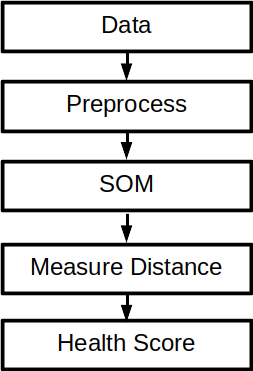
\includegraphics[width=4cm]{steps}
    \centering
    \label{fig:steps}
    \caption{Implementation steps from Data.}
\end{figure}